% TODO checklist:
% - [x] Inspected src/ directory structure via list_dir
% - [x] Inspected db/ directory structure for data layer organization
% - [x] Inspected tests/ directory structure for test organization
% - [x] Inspected ui_agent/ and ui_control_panel/ directories
% - [x] Read src/app.py for application factory pattern
% - [x] Read src/config.py for configuration organization
% - [x] Referenced README.md for project structure documentation
% - [x] Referenced Q&A.md Q9 for router modules, Q44 for test categories

\section{Codebase Structure}
\label{sec:codebase}

The Cineca Agentic Platform codebase follows a modular, layered architecture with clear separation between application logic, data access, presentation, and infrastructure concerns. This section documents the directory organization, key entry points, and module dependencies.

\subsection{Project Root Organization}

The repository root contains the following primary directories and configuration files:

\begin{verbatim}
cineca-agentic-platform/
├── src/                    # Main application source code
├── db/                     # Database layer (PostgreSQL, Redis, Memgraph)
├── tests/                  # Test suite (27 categories)
├── ui_agent/               # Next.js chat interface
├── ui_control_panel/       # Streamlit admin interface
├── ops/                    # Operations configurations
├── docs/                   # Documentation
├── api/                    # OpenAPI specifications
├── scripts/                # Utility scripts
├── docker-compose.yml      # Container orchestration
├── Dockerfile              # Application container definition
├── pyproject.toml          # Python project configuration
├── requirements.txt        # Runtime dependencies
└── README.md               # Project documentation
\end{verbatim}

\subsection{Source Code Organization (\texttt{src/})}

The \texttt{src/} directory contains the FastAPI application and all backend business logic, organized into functional modules:

\begin{table}[ht]
\centering
\caption{Source code directory structure and responsibilities.}
\label{tab:src-structure}
\small
\begin{tabular}{lp{8cm}}
\hline
\textbf{Directory} & \textbf{Purpose} \\
\hline
\texttt{routers/} & HTTP endpoint handlers (23 router modules) \\
\texttt{services/} & Business logic and orchestration \\
\texttt{mcp/} & Model Context Protocol tool implementations \\
\texttt{security/} & Authentication, authorization, and data protection \\
\texttt{schemas/} & Pydantic request/response models \\
\texttt{adapters/} & External system adapters (LLM, Memgraph) \\
\texttt{middleware/} & HTTP middleware components \\
\texttt{observability/} & Metrics, tracing, and monitoring \\
\texttt{background/} & Scheduled tasks and background jobs \\
\texttt{health/} & Health probe implementations \\
\texttt{jobs/} & Job models and store interfaces \\
\texttt{workers/} & Background job worker processes \\
\texttt{utils/} & Utility functions and helpers \\
\texttt{metrics/} & Prometheus metric definitions \\
\texttt{resilience/} & Circuit breaker and fallback logic \\
\hline
\end{tabular}
\end{table}

\subsubsection{Router Modules}

The \texttt{src/routers/} directory contains 23 FastAPI router modules organized by domain:

\begin{table}[ht]
\centering
\caption{Router modules by domain category.}
\label{tab:router-modules}
\small
\begin{tabular}{llp{5cm}}
\hline
\textbf{Domain} & \textbf{Module} & \textbf{Endpoints} \\
\hline
\multirow{3}{*}{Agent} 
    & \texttt{agents.py} & Agent sessions and runs \\
    & \texttt{agent\_runs.py} & Individual run operations \\
    & \texttt{agent.py} & Agent lifecycle management \\
\hline
\multirow{2}{*}{Jobs}
    & \texttt{jobs.py} & Job CRUD and status \\
    & \texttt{admin\_jobs.py} & Administrative job operations \\
\hline
\multirow{4}{*}{Models}
    & \texttt{models.py} & Model queries \\
    & \texttt{model\_instances.py} & Model instance configuration \\
    & \texttt{model\_management.py} & Provider management \\
    & \texttt{manifests.py} & Built-in model manifests \\
\hline
\multirow{4}{*}{Admin}
    & \texttt{tenants\_admin.py} & Multi-tenant management \\
    & \texttt{admin\_db.py} & Database administration \\
    & \texttt{admin\_ops.py} & Administrative operations \\
    & \texttt{admin.py} & Admin utilities \\
\hline
\multirow{2}{*}{Infrastructure}
    & \texttt{health.py} & Health probes (live/ready/startup) \\
    & \texttt{health\_v2.py} & Enhanced health endpoints \\
\hline
Other & \texttt{tools.py}, \texttt{auth.py}, \texttt{batch.py}, etc. & Tool discovery, authentication, bulk operations \\
\hline
\end{tabular}
\end{table}

\subsubsection{Service Layer}

The \texttt{src/services/} directory contains the core business logic:

\begin{table}[ht]
\centering
\caption{Key service modules and their responsibilities.}
\label{tab:service-modules}
\small
\begin{tabular}{lrl}
\hline
\textbf{Module} & \textbf{Lines} & \textbf{Responsibility} \\
\hline
\texttt{orchestrator.py} & 8,263 & Agent run execution engine \\
\texttt{intent\_classifier.py} & $\sim$500 & Intent mode classification \\
\texttt{default\_model\_resolver.py} & $\sim$400 & DMR with caching \\
\texttt{jobs\_service.py} & $\sim$350 & Job lifecycle management \\
\texttt{session.py} & $\sim$300 & Session state management \\
\texttt{archive.py} & $\sim$250 & Backup and restoration \\
\hline
\end{tabular}
\end{table}

\subsubsection{MCP Tools Structure}

The \texttt{src/mcp/tools/} directory contains 34 MCP tools organized into 17 categories:

\begin{verbatim}
src/mcp/tools/
├── admin/              # Administrative operations
├── agent/              # Agent context management
├── cache/              # Cache operations
├── catalog/            # Service discovery
├── data/               # Data quality and archival
├── db/                 # Database utilities
├── errors/             # Error reporting
├── graph/              # Graph queries and analytics
├── model/              # Model management
├── output/             # Response formatting
├── privacy/            # Privacy consent management
├── ratelimit/          # Rate limit operations
├── security/           # Security validation
├── session/            # Session lifecycle
├── system/             # System health and metrics
├── tenancy/            # Tenant operations
├── user/               # User profile management
└── viz/                # Visualization rendering
\end{verbatim}

\subsection{Database Layer (\texttt{db/})}

The \texttt{db/} directory contains all database-related code, organized by database type:

\begin{table}[ht]
\centering
\caption{Database layer directory structure.}
\label{tab:db-structure}
\small
\begin{tabular}{lp{8cm}}
\hline
\textbf{Directory} & \textbf{Contents} \\
\hline
\texttt{postgres\_control/} & SQLAlchemy models, Alembic migrations (26 versions), repository classes \\
\texttt{redis\_cache/} & Redis client wrappers, job store, rate limiting, caching utilities \\
\texttt{memgraph\_domain/} & Memgraph client, graph population scripts, sample queries \\
\texttt{migrations/} & Legacy SQL migration scripts \\
\hline
\end{tabular}
\end{table}

\subsubsection{PostgreSQL Schema}

The \texttt{db/postgres\_control/models/} directory defines SQLAlchemy ORM models:

\begin{table}[ht]
\centering
\caption{PostgreSQL model definitions.}
\label{tab:postgres-models}
\small
\begin{tabular}{ll}
\hline
\textbf{Model File} & \textbf{Entity} \\
\hline
\texttt{tenant.py} & Tenant configuration and isolation \\
\texttt{provider.py} & LLM provider definitions \\
\texttt{model\_instance.py} & Model instance configurations \\
\texttt{agent\_run.py} & Agent run records and metrics \\
\texttt{agent\_session.py} & Conversational session state \\
\texttt{agent\_step.py} & Individual execution steps \\
\texttt{job.py} & Background job definitions \\
\texttt{job\_event.py} & Job event stream records \\
\texttt{audit\_log.py} & Append-only audit trail \\
\texttt{tool\_invocation.py} & Tool call records \\
\hline
\end{tabular}
\end{table}

\subsubsection{Repository Pattern}

The \texttt{db/postgres\_control/repositories/} directory implements the repository pattern for data access:

\begin{lstlisting}[language=Python, caption={Repository pattern implementation example.}]
# db/postgres_control/repositories/agents.py
class AgentRunRepository:
    """Repository for agent run persistence."""
    
    def create(self, session: Session, run_data: dict) -> AgentRun:
        """Create new agent run record."""
        run = AgentRun(**run_data)
        session.add(run)
        session.commit()
        return run
    
    def get_by_id(self, session: Session, run_id: str) -> AgentRun | None:
        """Retrieve agent run by ID."""
        return session.query(AgentRun).filter(
            AgentRun.id == run_id
        ).first()
    
    def list_by_tenant(
        self, session: Session, tenant_id: str, 
        page_size: int = 50, page_token: str | None = None
    ) -> tuple[list[AgentRun], str | None]:
        """List runs for tenant with pagination."""
        # Tenant-scoped query implementation
\end{lstlisting}

\subsection{Test Suite Organization (\texttt{tests/})}

The test suite is organized into 27 category directories with comprehensive coverage:

\begin{table}[ht]
\centering
\caption{Test suite organization by category.}
\label{tab:test-categories}
\small
\begin{tabular}{llr}
\hline
\textbf{Category} & \textbf{Directory} & \textbf{Focus Area} \\
\hline
Unit tests & \texttt{tests/unit/} & Pure logic validation \\
Integration & \texttt{tests/integration/} & Service interaction \\
End-to-end & \texttt{tests/e2e/} & Full workflow validation \\
Security & \texttt{tests/security/} & Auth, RBAC, rate limits \\
Performance & \texttt{tests/performance/} & Latency benchmarks \\
API contracts & \texttt{tests/api/} & OpenAPI compliance \\
Health probes & \texttt{tests/health/} & Probe behavior \\
MCP tools & \texttt{tests/mcp/} & Tool invocation \\
Jobs & \texttt{tests/jobs/} & Job lifecycle \\
Agents & \texttt{tests/agents/} & Agent orchestration \\
\hline
\end{tabular}
\end{table}

The test suite statistics demonstrate comprehensive coverage:

\begin{itemize}
    \item \textbf{272 test files} across 27 categories
    \item \textbf{$\sim$64,500 lines} of test code
    \item \textbf{2,700+ test functions} covering all platform layers
    \item \textbf{60\% minimum coverage threshold} enforced in CI
\end{itemize}

\subsection{Key Entry Points}
\label{subsec:key-entry-points}

Understanding the platform's entry points is essential for developers working with or extending the codebase.

\subsubsection{Application Entry Point}

The primary application entry point is \texttt{src/app.py}, which provides the FastAPI application factory:

\begin{lstlisting}[language=Python, caption={Application factory responsibilities.}]
# src/app.py - Key responsibilities:
# 1. Initialize structured logging (structlog)
# 2. Install log masking for sensitive data
# 3. Validate secrets on startup
# 4. Create FastAPI instance with middleware
# 5. Mount routers for all API versions
# 6. Configure CORS and security headers
# 7. Initialize Prometheus metrics endpoint
# 8. Start background scheduler
\end{lstlisting}

\subsubsection{Orchestrator Engine}

The agent orchestration engine resides in \texttt{src/services/orchestrator.py}:

\begin{lstlisting}[language=Python, caption={Orchestrator entry points.}]
# src/services/orchestrator.py - Key methods:
class Orchestrator:
    async def run(
        self, 
        prompt: str,
        session_id: str | None = None,
        model_id: str | None = None,
        temperature: float = 0.7,
        max_steps: int = 10,
    ) -> AgentRunResult:
        """Execute a complete agent run with planning and steps."""
        
    async def _classify_intent(self, prompt: str) -> IntentResult:
        """Determine processing mode (CHAT, GRAPH, ADMIN, etc.)."""
        
    async def _execute_step(self, step: StepDefinition) -> StepResult:
        """Execute a single orchestration step."""
\end{lstlisting}

\subsubsection{Router Registration}

Routers are mounted in the application factory following a versioned pattern:

\begin{lstlisting}[language=Python, caption={Router registration pattern from \texttt{src/app.py}.}]
# Router mounting follows consistent versioning
from src.routers import (
    health, auth, agents, agent_runs, jobs,
    tools, tenants_admin, model_instances,
    model_management, admin_db, admin_ops
)

# v1 API endpoints
app.include_router(health.router, prefix="/v1", tags=["health"])
app.include_router(auth.router, prefix="/v1", tags=["auth"])
app.include_router(agents.router, prefix="/v1", tags=["agents"])
app.include_router(jobs.router, prefix="/v1", tags=["jobs"])
app.include_router(tools.router, prefix="/v1", tags=["tools"])
# ... additional routers
\end{lstlisting}

\subsubsection{Worker Entry Point}

The background job worker has its own entry point in \texttt{src/workers/jobs\_worker.py}:

\begin{lstlisting}[language=Python, caption={Worker process entry point.}]
# src/workers/jobs_worker.py
class JobsWorker:
    """Background job processor with heartbeat and graceful shutdown."""
    
    async def start(self):
        """Start the worker polling loop."""
        self._running = True
        while self._running:
            job = await self._poll_queue()
            if job:
                await self._process_job(job)
            await self._heartbeat()
    
    async def stop(self):
        """Graceful shutdown - complete current job first."""
        self._running = False
        await self._wait_for_current_job()
\end{lstlisting}

\subsubsection{Security Module Entry Points}

Security functionality is centralized in \texttt{src/security/}:

\begin{table}[ht]
\centering
\caption{Security module entry points.}
\label{tab:security-modules}
\small
\begin{tabular}{ll}
\hline
\textbf{Module} & \textbf{Entry Points} \\
\hline
\texttt{jwt.py} & \texttt{validate\_token()}, \texttt{extract\_claims()} \\
\texttt{auth.py} & \texttt{get\_current\_user()}, \texttt{require\_scopes()} \\
\texttt{authorization.py} & \texttt{check\_permission()}, \texttt{expand\_role\_scopes()} \\
\texttt{rate\_limit.py} & \texttt{check\_rate\_limit()}, \texttt{RateLimitMiddleware} \\
\texttt{pii\_scrubber.py} & \texttt{scrub()}, \texttt{detect\_pii()} \\
\texttt{output\_guard.py} & \texttt{guard()}, \texttt{OutputGuardMiddleware} \\
\hline
\end{tabular}
\end{table}

\subsubsection{MCP Tool Registry}

Tools are discovered and registered through the MCP runtime:

\begin{lstlisting}[language=Python, caption={MCP tool discovery mechanism.}]
# src/mcp/tools/__init__.py
def module_name_for_tool(tool_name: str) -> str:
    """Translate 'graph.query' -> 'src.mcp.tools.graph.query'"""
    return f"src.mcp.tools.{tool_name}"

def load(tool_name: str) -> tuple[ModuleType, Callable | None]:
    """Load tool module and find invoke function."""
    mod = importlib.import_module(module_name_for_tool(tool_name))
    _, fn = find_callable_in_module(mod)  # Looks for invoke, run, handle
    return mod, fn
\end{lstlisting}

\subsection{Module Dependencies}

The codebase follows a layered dependency structure to maintain clean separation of concerns:

\begin{figure}[ht]
\centering
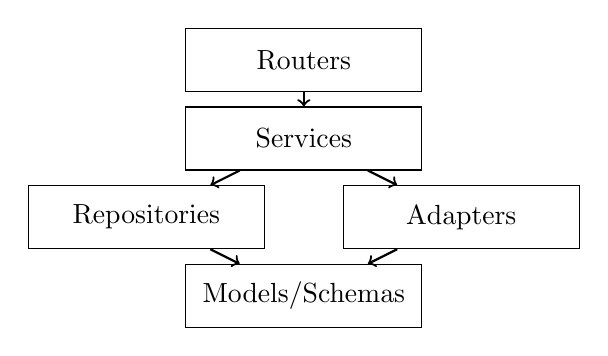
\begin{tikzpicture}[
    box/.style={rectangle, draw, minimum width=3cm, minimum height=0.8cm, align=center},
    arrow/.style={->, thick}
]
    % Layers
    \node[box] (routers) at (0, 3) {Routers};
    \node[box] (services) at (0, 2) {Services};
    \node[box] (repos) at (-2, 1) {Repositories};
    \node[box] (adapters) at (2, 1) {Adapters};
    \node[box] (models) at (0, 0) {Models/Schemas};
    
    % Dependencies
    \draw[arrow] (routers) -- (services);
    \draw[arrow] (services) -- (repos);
    \draw[arrow] (services) -- (adapters);
    \draw[arrow] (repos) -- (models);
    \draw[arrow] (adapters) -- (models);
\end{tikzpicture}
\caption{Module dependency hierarchy.}
\label{fig:module-deps}
\end{figure}

Key dependency rules enforced in the codebase:

\begin{enumerate}
    \item \textbf{Routers} depend on \textbf{Services} but not directly on repositories
    \item \textbf{Services} orchestrate between repositories and adapters
    \item \textbf{Repositories} abstract database access behind consistent interfaces
    \item \textbf{Adapters} handle external system communication (LLM, Memgraph)
    \item \textbf{Models/Schemas} are dependency-free data structures
\end{enumerate}

\subsection{Naming Conventions}

The codebase follows consistent naming conventions to improve discoverability:

\begin{table}[ht]
\centering
\caption{File and module naming conventions.}
\label{tab:naming-conventions}
\small
\begin{tabular}{lll}
\hline
\textbf{Type} & \textbf{Pattern} & \textbf{Example} \\
\hline
Router modules & \texttt{<domain>.py} & \texttt{agents.py}, \texttt{jobs.py} \\
Service modules & \texttt{<domain>\_service.py} & \texttt{jobs\_service.py} \\
Repository modules & \texttt{<domain>\_repo.py} & \texttt{model\_instance\_repo.py} \\
Schema modules & \texttt{<domain>.py} & \texttt{schemas/agents.py} \\
Test files & \texttt{test\_<module>.py} & \texttt{test\_agents.py} \\
MCP tools & \texttt{<category>/<action>.py} & \texttt{graph/query.py} \\
\hline
\end{tabular}
\end{table}

